\documentclass[11pt,letterpaper]{article}

% Load some basic packages that are useful to have
% and that should be part of any LaTeX installation.
%
% be able to include figures
\usepackage{graphicx}
% get nice colors
\usepackage{xcolor}

% change default font to Palatino (looks nicer!)
\usepackage[latin1]{inputenc}
\usepackage{mathpazo}
\usepackage[T1]{fontenc}
% load some useful math symbols/fonts
\usepackage{latexsym,amsfonts,amsmath,amssymb}

% comfort package to easily set margins
\usepackage[top=1in, bottom=1in, left=1in, right=1in]{geometry}
\usepackage{hyperref}
\usepackage[all]{hypcap}
% control some spacings
%
% spacing after a paragraph\begin{figure}[bth]
\setlength{\parskip}{.15cm}
% indentation at the top of a new paragraph
\setlength{\parindent}{0.0cm}

\begin{document}

\begin{center}
\Large
Ay190 -- Worksheet 06\\
David Vartanyan\\
Date: \today
\end{center}

\section{Exercise 1}

\subsection{a}


My function equivalent of dft(x) is labeled f(x), the Fourier transform of x. By running the hashtag lines, we see that f(x) is identical to g(x), the machine definition of the Fourier transform of x using numpy.fft.fft(x).

\subsection{b} \label{sec:b}

We run timeit to find the time it takes to run f(x) ten times on a random vector of the length N. I create and plot an array of N vs the time to run f(x), where $N=range(10,110,10)$.

Interestingly, I find that the time to run f(x) scales as N, not as $N^2$. This may be due to my stepwise definition of f(x). Since I define f(x) with all the subvariables (w(N), k, b) pre-defined, I wondered if this would affect the time to call f(x). However, after redefining f(x) to encompass all subvariables, I still got a linear fit of timeit with respect to N.

\subsection{c}

See Figure~\ref{fig:1}. I plot the results for f(x) and g(x) on two differently scaled y-axes. Note how g(x) takes several orders of magnitude less time to run and further does not depend on N as stiffly, illustrating the $N log N$ convergence for the fast Fourier transform. 

\subsection{d}

One way I made my code faster is referenced in Section~\ref{sec:b}. I simply redefined f(x) so that all the subvariables (e.g. w(N), k, b) were defined separately so calling f(x) was faster. Bending the rules? Sure. Returning a faster evaluation of f(x)? Definitely. For everything else, there's MasterCard.

\begin{figure}[bth]
\centering
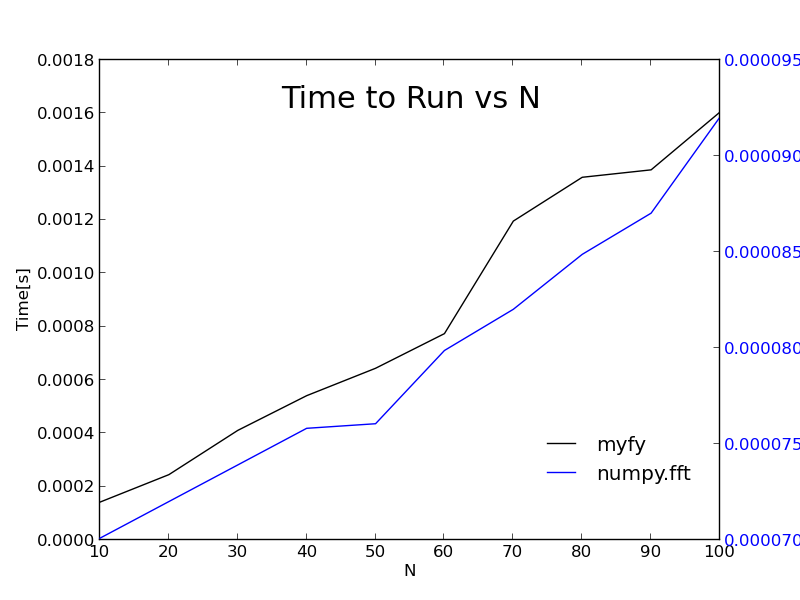
\includegraphics[width=0.7\textwidth]{ws6fig.png}
\caption{Timeit vs N.}
\label{fig:1}
\end{figure}

\end{document}
